\IfFileExists{ajr.sty}
{\documentclass[12pt]{article}
\usepackage[a5paper,margin=5mm]{geometry}}
{\documentclass[12pt,a4paper]{article}}

\usepackage{url,natbib}
\let\harvardurl\url
\usepackage{graphicx,subcaption}
\usepackage{amsmath,amsfonts,defns}
\usepackage{pgfplots}

\newcommand{\Bb}[1]{%
  \expandafter\def\csname#1#1\endcsname%
  {\ensuremath{\mathbb #1}}}
\Bb X\Bb T\Bb R\Bb I\Bb J
\newcommand{\secref}[1]{\ref{sec:#1}}

\title{An application of piecewise-linear holistic discretisation}
\author{G.~A. Jarrad and A.~J. Roberts}

\begin{document}
\maketitle

\begin{abstract}
The fidelity of numerical simulation of a spatio-temporal dynamical system is 
largely constrained by the chosen discretisation of the PDE. 
In particular, the modeller is typically free to choose
arbitrary finite-element forms for the various spatial derivatives,
without necessarily having knowledge of the accuracy of the resulting numerical schemes.
The holistic discretisation approach described in this paper obviates the problem of arbitration. % mediation?

Centre manifold theory is applied to derive an asymptotically accurate
representation of the microscale dynamics of the one-dimensional Burgers' equation. 
In the process, the corresponding macroscale dynamics 
are constrained to match the microscale solution at discrete grid-points.
The resulting representation of macroscale evolution provides an unambiguous discretisation of the PDE,
suitable for numerical simulation. 

The iterative process starts with a choice of the leading, macroscale approximation to the linearised system.
Suitable internal boundary conditions are then induced on the spatial derivatives 
at the end-points of each discrete interval.
Although the choice of IBCs might appear to be arbitrary, they are in fact governed by the placement of the grid-points and the 
form of the leading discrete approximation.
The particular approach taken here is to start with a piecewise linear but continuous approximation,
in contrast to similar analyses that use piecewise constant, discontinuous approximations.
This is motivated by the principle that a more accurate leading approximation should lead to faster
convergence of the asymptotic solution, via the Rayleigh-Ritz theorem.

Further iterations of the centre manifold process lead inexorably to a temporal evolution formulation of the macroscale dynamics,
holistically informed by the underlying microscale dynamics.  
We examine the accuracy and stability of the resulting numerical scheme, in comparison to
the behaviours of several other typical approximations.
\end{abstract}

\numberwithin{equation}{section}
\numberwithin{figure}{section}
\numberwithin{table}{section}
\section{Introduction}\label{sec:intro}
As an application of holistic discretisation, consider the numerical simulation of a field~\(u(x,t)\) of the nonlinear advection--diffusion Burgers' \pde
\begin{eqnarray}
	\D tu = \nu\DD xu - \alpha u\D xu\,.
\label{eq:burgers}
\end{eqnarray}
%Mention cole-hopf leads to known solution which is unconditionally stable.
The spatial domain~\(\XX\) is of length~\(L\), \(0\leq x\leq L\)\,, and we consider solutions \(L\)-periodic in space.
The first step is to discretise $\XX$ into $N$ equi-spaced intervals bounded by $N+1$~grid-points~\(X_j\), \({j=0,\ldots,N}\), with spacing~\(H\).
The continuum dynamics of the field~$u(x,t)$ are now summarised by the coarse dynamics
${\vec U}=(U_1,U_2,\ldots,U_N)$, where $U_j(t):=u(X_j,t)$ for all $t\in \TT$.

The next step is to specify the explicit form of the coarse temporal evolution
\begin{eqnarray}
	\dot{\vec U}(t) = {\vec g}({\vec U}(t))\,.
\label{eq:temporal}
\end{eqnarray}
The traditional approach is to use centred approximations, for example, $\delta^2 U_j/H^2$ for $\DD xu$
and $U_j\mu\delta U_j/H$ for $u\D xu$, 
where $\delta=\sigma^{\frac{1}{2}}-\sigma^{-\frac{1}{2}}$,
$\mu=(\sigma^{\frac{1}{2}}+\sigma^{-\frac{1}{2}})/2$,
and $\sigma U_j=U_{j+1}$.
However, the advection term has another plausible representation, namely the
conservative form $\mu\delta U_j^2/2H$.
For illustrative purposes, a mixture of the two latter representations will be used for comparison,
namely
\begin{eqnarray}
	\dot{U}_j = \nu\frac{\delta^2 U_j}{H^2}-(1-\theta)\alpha\frac{U_j\mu\delta U_j}{H}
-\theta\alpha\frac{\mu\delta U_j^2}{2H}\,.
\label{eq:mixture}
\end{eqnarray}
In contrast, the holistic approach has no such representational ambiguity, and, 
as shown in Section~\secref{nonlin}, gives rise at first-order to the model
\begin{eqnarray}
	\dot{U}_j = S\left(\nu\frac{\delta^2 U_j}{H^2}-\alpha\frac{U_j\mu\delta U_j}{3H}
-\alpha\frac{\mu\delta U_j^2}{3H}\right)\,,
\label{eq:holistic1}
\end{eqnarray}
where $S=(1+\delta^2/6)^{-1}$. Observe that, apart from the non-local corrective operator $S$,
this holistic model matches the mixture model~\eqref{eq:mixture} for $\theta=\frac{2}{3}$.
This parameter value is exactly the critical value predicted by \cite{Fornberg73}
to be necessary for stable simulation (with $\nu=0$ and $\alpha=1$) for a selection of numerical integration schemes.
Further comparisons of the numerical behaviours of the holistic and mixture models are given in Section~\secref{numeric}.

The final step in the simulation process is to interpolate  from the coarse solution ${\vec U}(t)$ 
back to the continuum field $u(x,t)$ via a spatial mapping of the form
\begin{eqnarray}
	u(x,t)  = \hat{u}(x,{\vec U}(t))\,.
	\label{eq:spatial}
\end{eqnarray}
The complete holistic framework comprises equations~\eqref{eq:temporal} and \eqref{eq:spatial},  along with the addition of suitable boundary conditions that are discussed in Section~\ref{sec:lin}.
We show in Section~\secref{nonlin} that, to first-order, the holistic mapping $\hat{u}$ takes the form
\begin{eqnarray}
\hat{u} = \sum_{j=1}^{N}\chi_j\left({\cal I}_{0}U_j+\frac{H^2}{6}{\cal I}_{1}\dot{U}_j
+\alpha\frac{H}{6}{\cal I}_{1}U_j\cdot (1-\sigma^{-1})U_j\right)\,,
\end{eqnarray}
using the interpolation operators ${\cal I}_{0}=\xi+(1-\xi)\sigma^{-1}$
and ${\cal I}_{1}=\xi^3+(1-\xi)^{3}\sigma^{-1}-\xi(1-\sigma^{-1})-\sigma^{-1}$,
where $\xi=\sum_{j=1}^{N}\chi_j\xi_j$ with $\xi_j(x)=(x-X_{j-1})/H$ 
and $\chi_j(x)=1$ (else $0$) for $X_{j-1}\le x<X_j$.

\section{Motivation}\label{sec:motive}
The choice of a piecewise linear leading approximation, in contrast to the usual piecewise constant one
 \cite[]{Roberts98a, Roberts00a, Roberts2011a}, is motivated by an application of the Rayleigh--Ritz theorem.
Consider a general dynamical system of the form
\begin{eqnarray}
\dot{\vec u} = {\cal L}{\vec u}+{\cal N}({\vec u})\,,
\label{eq:nonlin:gen}
\end{eqnarray}
where it is pre-supposed for convenience that ${\cal N}({\vec 0})={\vec 0}$. 
The slow manifold approximation to the dynamics of the linearised system
\begin{eqnarray}
 \dot{{\vec u}}={\cal L}{\vec u}
\label{eq:lin:gen}
\end{eqnarray}
about ${\vec u}={\vec 0}$ is then parameterised as
\begin{eqnarray}
{\vec u} = V{\vec s}\,, && \dot{{\vec s}} = \Lambda{\vec s}\,,
\end{eqnarray}
whereupon $V\Lambda{\vec s}={\cal L}V{\vec s}$ for arbitrary ${\vec s}$.
Observe now that a particular choice of $\Lambda=\mbox{diag}(\lambda_1,\lambda_2,\ldots)$ uncouples this relation into the components
${\cal L}{\vec v}_j=\lambda{\vec v}_j$, where $V=\left[{\vec v}_1,{\vec v}_2,\ldots\right]$.

Now, when ${\cal L}$ is self-adjoint, the Rayleigh--Ritz theorem is that $\lambda_j = R({\vec v}_j)$ for the Rayleigh quotient 
\[ R({\vec v}) = \frac{\langle{\vec v},{\cal L}{\vec v}\rangle}{\|{\vec v}\|^2}\,.\]
 It can further be shown, upon perturbing ${\vec v}_j$ to ${\vec u}={\vec v}_j+\epsilon{\vec w}$,
that $R({\vec u})=\lambda_j+O(\epsilon^2)$.
%This provides support for the general expansions
%\begin{eqnarray}
%{\vec u} \sim V{\vec s}+\epsilon{\vec w}_1+\epsilon^2{\vec w}_2+\ldots\,,
%&& 
%\dot{\vec u} \sim V\Lambda{\vec s}+\epsilon{\vec g}_1+\epsilon^2{\vec g}_2+\ldots\,,
%\end{eqnarray}
%for the nonlinear dynamical system~\eqref{eq:nonlin:gen}.
The slow manifold is based upon the slow subspace spanned by the slow eigenvectors, and the evolution on the slow manifold corresponds to eigenvalues of the linearisation.
Hence the Rayleigh--Ritz quotient suggests that the more accurate we make a linear subspace approximation to the field~\(u(x,t)\), the more accurate the evolution on the slow manifold.
Consequently, Section~\ref{sec:lin} develops a piecewise linear and continuous subspace approximation to the field, instead of the piecewise constant and discontinuous approximation developed previously \cite[]{Roberts98a, Roberts00a, Roberts2011a}.

\section{Linear analysis}\label{sec:lin}
Burgers' equation~\eqref{eq:burgers} linearises to equation~\eqref{eq:lin:gen} for $\alpha=0$, with the linear operator
${\cal L}=\nu\DD x{}$. It can be shown that ${\cal L}$ is self-adjoint under any of these external boundary conditions:
\(L\)-periodic; Dirichlet ($u(0,t)=u(L,t)=0$); or Neuman ($u_x(0,t)=u_x(L,t)=0$). We have chosen the first
condition for convenience.
The linear system has two eigenmodes corresponding to eigenvalue $\lambda=0$, namely
\begin{eqnarray}
  v = 1\,, && v = x\,, 
\end{eqnarray}
and general eigenmodes for $\lambda=-\nu k^2<0$ of the form
\begin{eqnarray}
 v = e^{-\nu k^2 t\pm ikx}\,.&&
\end{eqnarray}
Hence, any peicewise--linear approximation to $u$ is an equilibrium solution of the linearised system.
We choose a continuous approximation that is aligned at the internal grid-points $X_j=jH$, $j=1,2,\ldots,N-1$, namely
\begin{eqnarray}
     \hat{u}_{0} = \sum_{j=1}^{N}\chi_j(\xi U_j+(1-\xi)U_{j-1})
% = \sum_{j=1}^{N}\chi_j(\xi+(1-\xi)\sigma^{-1})U_j
\,,
\label{eq:uhat0}
\end{eqnarray}
with indicator $\chi_j(x)=1$ (else 0) for $X_{j-1}\le x<X_j$, and dimensionless coordinate
$\xi(x)=\sum_{j=1}^{N}\chi_j(x)(x-X_{j-1})/H$. This enforced continuity is represented by internal boundary conditions
(IBCs) of the form 
\begin{eqnarray}
   [\hat{u}]_j = 0 && \mbox{for } j=1,2,\ldots,N-1\,,
\label{eq:cont-cond}
\end{eqnarray}
where $ [u]_j := \lim_{\epsilon\rightarrow 0^{+}} u(X_j+\epsilon,t)-u(X_j-\epsilon,t)$
represents the spatial jump in $u$ across the boundary between the $j$-th and $(j+1)$-th intervals.

Unfortunately, this continuity does not hold for the first spatial derivative, since it can be shown that
$[\D x{\hat{u}_{0}}]_j=\delta^2U_j/H$. Hence, we introduce a homotopic smoothing parameter $\gamma$
($0\le\gamma\le 1$),
and enforce the additional IBCs: %smoothness condition that
\begin{eqnarray}
   [\hat{u}_x]_j = \frac{1-\gamma}{H}\left.\delta^2\hat{u}\right|_{X_j} && \mbox{for } j=1,2,\ldots,N-1\,,
\label{eq:smooth-cond}
\end{eqnarray}
such that smooth approximations are found in the limit as $\gamma\rightarrow 1$.
Consequently, the state-space is now extended to $(u,\alpha,\gamma)$, for which $(\hat{u}_{0},0,0)$ is
an equilibrium of equation~\eqref{eq:burgers}.  

We now demonstrate that the system will be robust to nonlinear perturbations about this equilibrium.
We seek the spatial stability over $\XX$ of the eigenmode
\begin{eqnarray}
v = \sum_{j=1}^{N}\chi_j \Re\left(a_j e^{i\kappa\xi}\right)\,,
\end{eqnarray}
for some fixed, nondimensionalised wavenumber $\kappa=kH$, and 
arbitrary, time--varying coefficients $a_j=A_j+iB_j$. 
The continuity condition~(\ref{eq:cont-cond}) now implies that
\begin{eqnarray}
\Re\left(a_{j+1} - a_j e^{i\kappa}\right) = 0\,.
\end{eqnarray}
Similarly, the smoothness condition~(\ref{eq:smooth-cond}) implies that 
\begin{eqnarray}
-\kappa \Im\left(a_{j+1} - a_j e^{i\kappa}\right) =  
(1-\gamma)\Re\left(a_{j+1} e^{i\kappa} + a_j - 2 a_j e^{i\kappa}\right)\,.
\end{eqnarray}
In coefficient form, the update from the $j$-th to $(j+1)$-th interval is
\begin{eqnarray}
\left[\begin{array}{cc}
1 & 0\\
fc & 1-fs\\
\end{array}\right]
\left[\begin{array}{c}
A_{j+1}\\
B_{j+1}\\
\end{array}\right]
=
\left[\begin{array}{cc}
c & -s\\
s+f(2c-1) & c-2fs\\
\end{array}\right]
\left[\begin{array}{c}
A_{j}\\
B_{j}\\
\end{array}\right]\,,
\end{eqnarray}
where $c+is=e^{i\kappa}$ and $f=(1-\gamma)/\kappa$.
Putting $a_{j+1}=\mu a_j$ then leads to the characteristic equation
\begin{eqnarray}
\mu^2-2\frac{c-fs}{1-fs}\mu+1 = 0\,,
\end{eqnarray}
with characteristic roots given by
\begin{eqnarray}
\mu & = & \beta\pm\sqrt{\beta^2-1}
\hspace*{5mm}\mbox{for } 
\beta~=~\frac{c-fs}{1-fs}\le 1\,.
\end{eqnarray}
Consequently, there are three distinct stability regimes governed by $\beta$:
\begin{enumerate}
\item $|\beta|<1$, which gives rise to complex roots with $|\mu|=1$ ({\em stable}). 
This includes the limiting case of $\gamma=1$ ($f=0$), for which
$\mu=c\pm is=e^{\pm i\kappa}$.

\item $\beta=\pm 1$, corresponding to $\kappa=n\pi$, $n=0,1,2,\ldots$, 
which gives rise to a repeated, real root of $\mu=\pm 1$ ({\em stable}).

\item $\beta<-1$, which gives rise to the two real roots $\mu<-1$ and $-1<\mu<0$
({\em saddle unstable}).
\end{enumerate}
The $\beta<-1$ regime comprises small regions of instability near $\kappa=(2n+1)\pi$,
$n=0,1,2,\ldots$, for which the eigenmode cannot persist unattenuated throughout space.
It can be shown that these forbidden regions obey
\begin{eqnarray}
\frac{\kappa}{2} <(1-\gamma)\tan\frac{\kappa}{2}\,, && \kappa\ne n\pi\,.
\label{eq:leaforbid}
\end{eqnarray}
Thus, at equilibrium ($\gamma=0$) there is an initial forbidden gap $\kappa\in(0,\pi)$ adjacent to the centre manifold
wavenumber $\kappa=0$ (see Figure~\ref{fig:leaspec}), indicating that transient solutions decay
 to the centre manifold at a rate of at least
$\lambda=-\nu k^2=-\frac{\nu\pi^2}{H^2}$. It is this gap that provides robustness to nonlinear perturbations
about the equilibrium within some suitable region in state-space.
\begin{figure}[hbt]
\centering
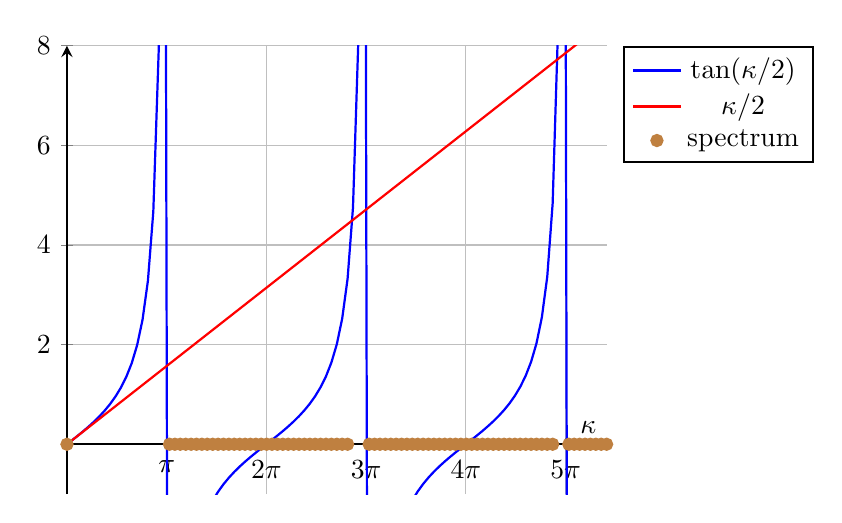
\begin{tikzpicture}
\begin{axis}[ xlabel={$\kappa$}
  ,axis x line=middle,axis y line=middle
  ,thick,grid,samples=101
  ,ymin=-1,ymax=8 ,domain=0:17
  ,xtick={3.1416,6.2832,9.4248,12.5664,15.7080}
  ,xticklabels={$\pi$,$2\pi$,$3\pi$,$4\pi$,$5\pi$}
  ,legend pos=outer north east
  ] 
\addplot [blue,no marks] {tan(deg(x)/2)}; 
\addlegendentry{$\tan(\kappa/2)$};
\addplot [red,no marks,samples=2] {x/2}; 
\addlegendentry{$\kappa/2$};
\addplot [brown,only marks,mark=*] {0-99*(x/2<tan(deg(x)/2))};
\addlegendentry{spectrum};
\end{axis}
\end{tikzpicture}
\caption{The equilibrium ($\gamma=0$, $\alpha=0$) spectrum
determined by the forbidding condition~\eqref{eq:leaforbid}.
The thick lines along the $\kappa$-axis indicate regions of wavenumbers
for which the corresponding eigenmodes are stable.}
\label{fig:leaspec}
\end{figure}


\section{Nonlinear analysis}\label{sec:nonlin}

With the aid of  holistic equations~\eqref{eq:temporal} and \eqref{eq:spatial}, 
viz $u=\hat{u}$ and $\dot{\vec{U}}=\vec{g}$, we rewrite
Burgers' equation~\eqref{eq:burgers} in the form
\begin{eqnarray}
 {\cal M}(\hat{u},\vec{g}) = {\cal L}\hat{u}-\D {\vec{U}}{\hat{u}}\cdot\vec{g}-\alpha\hat{u}\hat{u}_{x} = 0\,,
\label{eq:man}
\end{eqnarray}
where ${\cal L}=\nu\DD {x}{}$ from Section~\ref{sec:lin}. The linear analysis of that section is now extended
by considering perturbations about the equilibrium $(\hat{u},\gamma,\alpha)=(\hat{u}_{0},0,0)$.
%, where$\hat{u}_{0}=\sum_{j=1}^{N}\chi_j{\cal I}_0 U_j$ with ${\cal I}_0=\xi+(1-\xi)\sigma^{-1}$.
In particular, consider the power series
\begin{eqnarray}
  \hat{u} \sim \sum_{p=0}^{\infty}\sum_{q=0}^{\infty}\gamma^{p}\alpha^{q}\hat{u}^{(p,q)}\,,
&&
  \vec{g} \sim \sum_{p=0}^{\infty}\sum_{q=0}^{\infty}\gamma^{p}\alpha^{q}\vec{g}^{(p,q)}\,,
\label{eq:power}
\end{eqnarray}
where $\hat{u}^{(0,0)}=\hat{u}_{0}$ 
and $\vec{g}^{(0,0)}=0$.
Substituting these expansions into
equation~\eqref{eq:man},  the terms $\hat{u}^{(p,q)}$ and $\vec{g}^{(p,q)}$ are computed
subject to the IBCs \eqref{eq:cont-cond} and \eqref{eq:smooth-cond}.

To simplify this process  algebraically, we follow the approach of Jarrad:
without loss of generality, consider finite truncations of the power series subject to $p+q\le n$,
namely\footnote{In practice, other truncation schemes may be used;
for example, rectangular truncation: $p\le n$, $q\le m$.}
\begin{eqnarray}
   \hat{u}^{<n>} = \sum_{p=0}^{n}\sum_{q=0}^{n-p}\gamma^{p}\alpha^{q}\hat{u}^{(p,q)}\,,
&&
   \hat{u}_n = \sum_{p=0}^{n}\gamma^{p}\alpha^{n-p}\hat{u}^{(p,n-p)}\,.
\end{eqnarray}
Letting $\varepsilon^2=\gamma^2+\alpha^2$ for convenience\footnote{
This is merely an algebraic device; in practice, $\gamma$ and $\alpha$ need not be commensurate}, we obtain
 $\hat{u}=\hat{u}^{<n>}+O(\varepsilon^{n+1})$ and
$\hat{u}^{<n>}=\hat{u}^{<n-1>}+\hat{u}_{n}$; 
likewise for $\vec{g}^{<n>}$ and $\vec{g}_n$.
It can then be shown that
\begin{eqnarray}
 {\cal M}(\hat{u}^{<n>},\vec{g}^{<n>}) = 
  {\cal L}\hat{u}_n-\D {\vec{U}}{\hat{u}_0}\cdot\vec{g}_n+{\cal M}(\hat{u}^{<n-1>},\vec{g}^{<n-1>})
+O(\varepsilon^{n+1})\,,
\end{eqnarray}
and hence the process is to iteratively solve
\begin{eqnarray}
 {\cal M}(\hat{u}^{<n>},\vec{g}^{<n>}) = 0+O(\varepsilon^{n+1})\,,
\end{eqnarray}
or, equivalently,
\begin{eqnarray}
{\cal L}\hat{u}_n = \D {\vec{U}}{\hat{u}_0}\cdot\vec{g}_n-{\cal M}(\hat{u}^{<n-1>},\vec{g}^{<n-1>})
%+O(\varepsilon^{n+1})
\,.
\label{eq:order-n}
\end{eqnarray}

Given $\hat{u}_0=\sum_{j=1}^{N}\chi_j(\xi+(1-\xi)\sigma^{-1})U_j$ 
where $\xi=\sum_{j=1}^{N}\chi_j(x-X_{j-1})/H$, the first-order pertubation terms 
can now be computed for $n=1$. Defining $\Delta=1-\sigma^{-1}$, observe that
\begin{eqnarray}
\nu\hat{u}_{1}'' = \sum_{j=1}^{N}\chi_j\left[(\xi+(1-\xi)\sigma^{-1})g_{1,j}
   +\alpha(\xi+(1-\xi)\sigma^{-1})U_j.\frac{1}{H}\Delta U_j\right]\,.
\end{eqnarray}
Hence, spatially integrating twice gives
%\begin{eqnarray}
%\nu\hat{u}_{1}' & = & \sum_{j=1}^{N}\chi_j\left[c_j+ \frac{H}{2}(\xi^2-(1-\xi)^2\sigma^{-1})g_{1,j}
%\right.
%\nonumber\\
%&&  \left.{}+\frac{\alpha}{2}(\xi^2-(1-\xi)^2\sigma^{-1})U_j.\Delta U_j\right]
%\end{eqnarray}
\begin{eqnarray}
\nu\hat{u}_{1} & = &  \sum_{j=1}^{N}\chi_j\left[d_j+H\xi c_j+\frac{H^2}{6}(\xi^3+(1-\xi)^3\sigma^{-1})g_{1,j}
\right.\nonumber\\
&& \left.{}+\frac{\alpha H}{6}(\xi^3+(1-\xi)^3\sigma^{-1})U_j.\Delta U_j\right]\,.
\end{eqnarray}
Now, the continuity condition~\eqref{eq:cont-cond} ensures that $\hat{u}_n(X_j,t)=0$ for $n>0$,
since $\hat{u}_{0}(X_j,t)=U_j(t)=u(X_j,t)$. Hence, we solve for $d_j$ at $\xi=0$ and
$c_j$ at $\xi=1$, giving
\begin{eqnarray}
\nu\hat{u}_{1} & = &  \sum_{j=1}^{N}\chi_j\left[\frac{H^2}{6}(\xi^3+(1-\xi)^3\sigma^{-1}
-\xi\Delta-\sigma^{-1})g_{1,j}
\right.\nonumber\\
&& \left.{}+\frac{\alpha H}{6}(\xi^3+(1-\xi)^3\sigma^{-1}-\xi\Delta-\sigma^{-1})U_j.\Delta U_j\right]\,.
\end{eqnarray}
It is convenient here to introduce interpolation operators, ${\cal I}_0=\xi+(1-\xi)\sigma^{-1}$ and
${\cal I}_1=\xi^3+(1-\xi)^3\sigma^{-1}-\xi\Delta-\sigma^{-1}$ (observe that ${\cal I}_1''=6{\cal I}_0/H^2$),
whence
\begin{eqnarray}
 \hat{u} = \sum_{j=1}^{N}\chi_j\left[{\cal I}_0 U_j+\frac{H^2}{6\nu}{\cal I}_1\dot{U}_j
+\frac{\alpha H}{6\nu}{\cal I}_1 U_j.\Delta U_j\right]+O(\gamma^2+\alpha^2)\,,
\end{eqnarray}
since $\dot{U}_j=g_{1,j}+O(\gamma^2+\alpha^2)$. 

Next, the value for $g_{1,j}$ can likewise be found
from the smoothness condition~\eqref{eq:smooth-cond}, namely
\begin{eqnarray}
\nu[\hat{u}_{1}']_{j} = -H\left(1+\frac{1}{6}\delta^2\right)g_{1,j} 
-\frac{\alpha}{3}\left(U_j.\mu\delta U_j+\mu\delta U_j^2\right)
= -\frac{\nu\gamma}{H}\delta^2 U_j\,,
\label{eq:g1}
\end{eqnarray}
giving
\begin{eqnarray}
  \dot{U}_j  = S\left[\frac{\nu\gamma}{H^2}\delta^2 U_j
-\frac{\alpha}{3H}U_j.\mu\delta U_j-\frac{\alpha}{3H}\mu\delta U_j^2
\right]+O(\gamma^2+\alpha^2)\,,
\end{eqnarray}
where $S=(1+\delta^2/6)^{-1}$ is a non-local smoothing operator.
Observe that, apart $S$, this is just the mixture model~\eqref{eq:mixture}
with $\theta=\frac{2}{3}$. It turns out that this parameter value is exactly the critical value predicted by \cite{Fornberg73}
to be a necessary condition for the stability of numerical integration of the mixture model with $\nu=0$ and $\alpha=1$.
We demonstrate in Section~\secref{numeric} how this stability arises in low-dimensional models.

Higher order terms in $\hat{u}_n$  may be systematically computed by iteratively solving equation~\eqref{eq:order-n} after
having first computed $\vec{g}_n$. The latter can be found by applying the weak solvability condition 
(see \cite{Jarrad2001}),
namely that the right-hand side of equation~\eqref{eq:order-n} must be orthogonal to the null-space of the adjoint
operator ${\cal L}^{\dagger}$. Since ${\cal L}$ is self-adjoint in this example, we can isolate the boundary between the
$j$-th and $(j+1)$-th intervals using the linear approximation
\begin{eqnarray}
  \hat{v}_0 = \chi_j\xi + \chi_{j+1}(1-\xi)\,,
\end{eqnarray}
which satisfies both the continuity condition~\eqref{eq:cont-cond} and the smoothness condition~\eqref{eq:smooth-cond}
(for $\gamma=0$). Thus, taking the inner product of equation~\eqref{eq:order-n} with $\hat{v}_0$ gives
rise to the solvability condition
\begin{eqnarray}
\left.\frac{\nu\gamma}{H}\delta^2\hat{u}_{n-1}\right|_{X_j} = HS^{-1}g_{n,j}
-\langle {\cal M}(\hat{u}^{<n-1>},\vec{g}^{<n-1>}), \hat{v}_0 \rangle\,.
\end{eqnarray}
For $n=1$, note that this just reduces to equation~\eqref{eq:g1}.

\section{Numerical stability}\label{sec:numeric}

\section{Conclusion}


\bibliographystyle{agsm}
\IfFileExists{ajr.sty}
{\bibliography{bibexport,bib,ajr}}
{\bibliography{bibexport,yourbibfile}}


\end{document}
